\chapter{Detector Performance}
\label{ch:fdsp-perform}

%%%%%%%%%%%%%%%%%%%%%%%%%%%%%%%%%%%%%%%%%%%%%%%%%%%%%%%%%%%%%%%%%%%%
\section{??}
\label{sec:fdsp-perform-??}

\section{Far Detector Optimization Studies}
\label{sec:fdsp-perform-optimization}

The DUNE Far Detector Task Force was formed in 2015 and charged with developing a complete simulation and reconstruction infrastructure, and using these tools in optimization studies of key detector parameters such as wire pitch and angle.  The final report of that task force was presented in 2017 and includes a number of results that help motivate the design of the DUNE-SP modules presented in this document.  Highlights from these optimization studies are presented in this section, and include comparisons of the following DUNE geometry arrangements:

\begin{itemize}
\item{\textbf{Default}: APAs with 5 mm wire pitch, and Induction wires at 36$^{\circ}$ angle.}
\item{\textbf{3mm}: APAs with 3 mm wire pitch, and Induction wires at 36$^{\circ}$ angle.}
\item{\textbf{45Deg}: APAs with 5 mm wire pitch, and Induction wires at 45$^{\circ}$ angle.}
\item{\textbf{r90DegBeam}: APAs with 5 mm wire pitch, and Induction wires at 36$^{\circ}$ angle, but with APAs effectively rotated 90 degrees from the beam axis.}  
\end{itemize}



\subsection{Tracking Efficiency}
\label{sec:fdsp-perform-trackingeff}



\begin{dunefigure}[Impact of APA geometry on muon/pion/proton tracking efficiency]{fig:fdsp-perform_trackingeff_optimization}{Tracking efficiency for $\mu^-$ (top-left), $\pi^+$ (top-right), $\pi^-$ (bottom-left), and $p$ (bottom-right) from charged-current interactions, shown for 4 arrangements of APA geometry.}
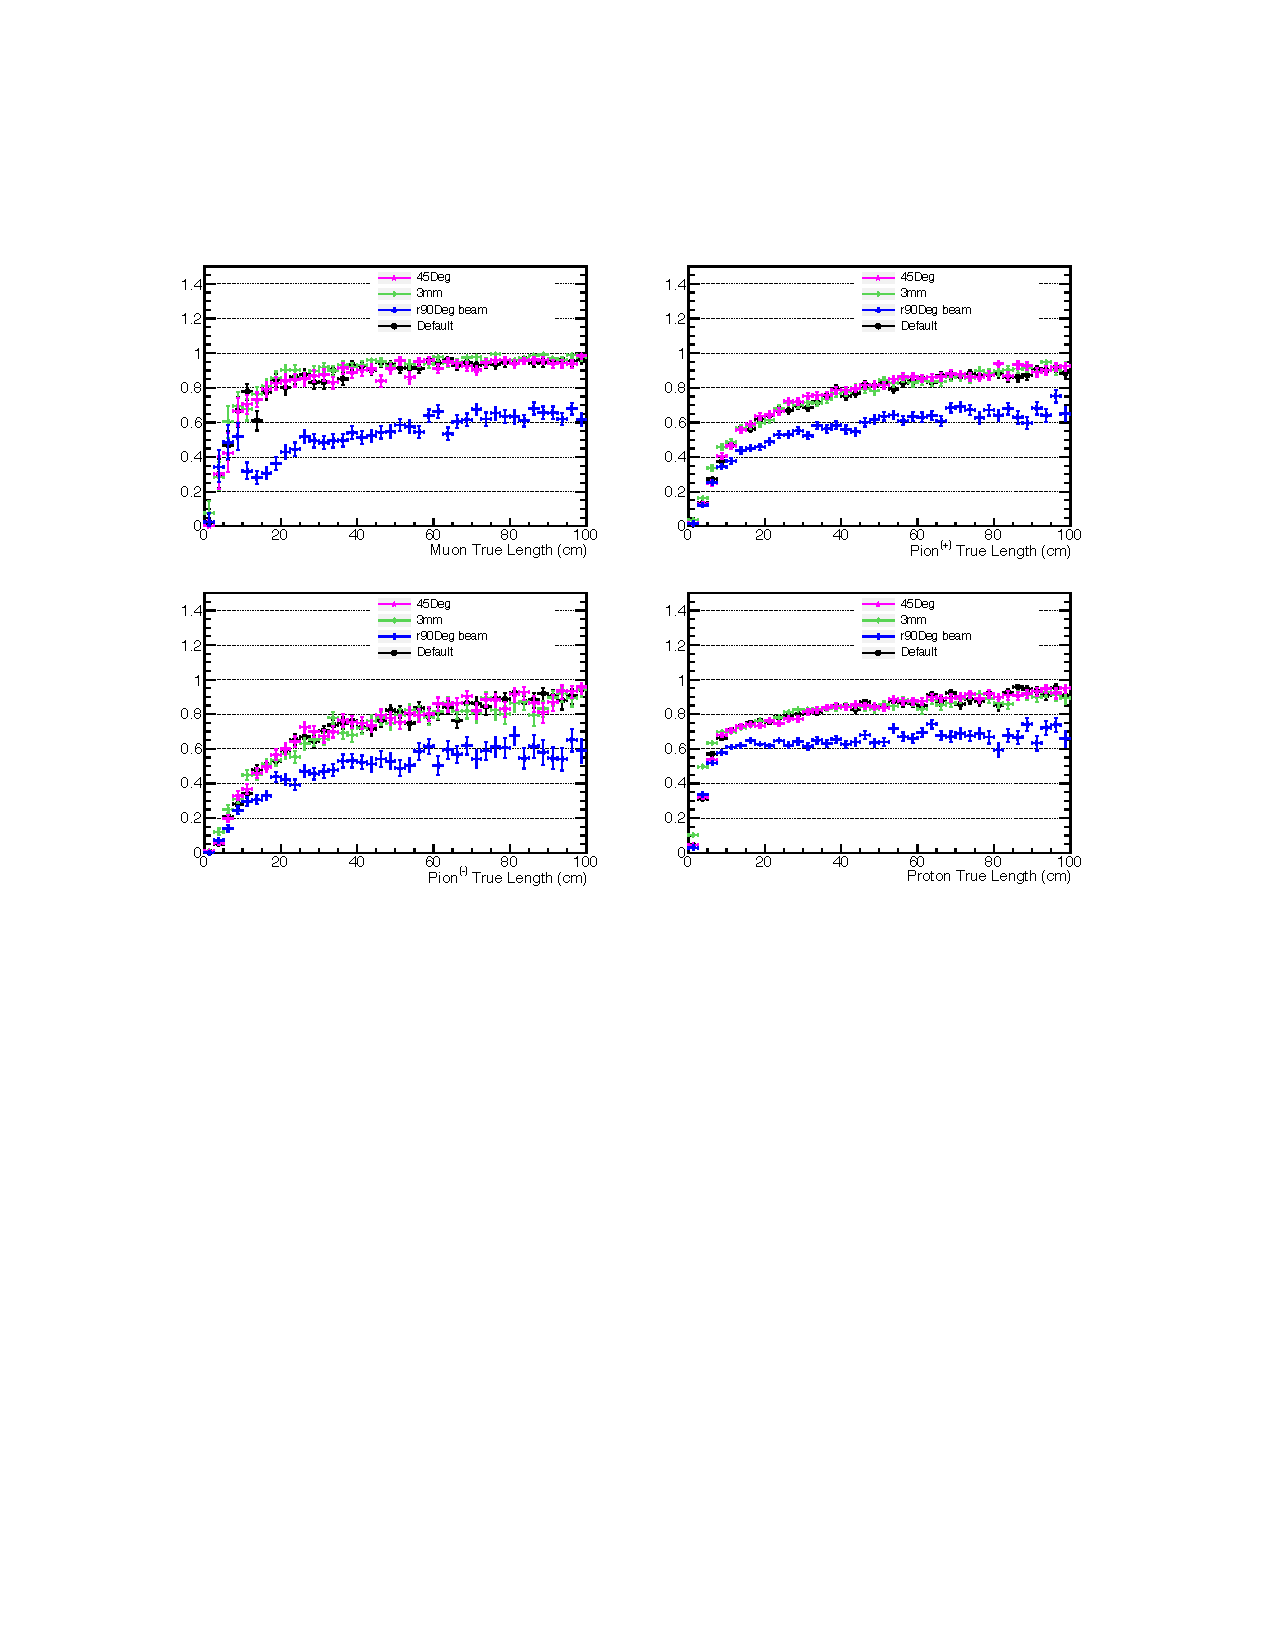
\includegraphics[width=0.85\textwidth]{TrackingEfficiency_GeometryOptimization.pdf}
\end{dunefigure}

\begin{dunefigure}[Tracking efficiency comparison between different reconstruction algorithms]{fig:fdsp-perform_trackingeff_comparison}{Tracking efficiency $K^+$ (top), $\mu^+$ (middle), and Michel electrons (bottom) using LineCluster (left) or TrajCluster (right), as a function of true particle length in proton decay events.}
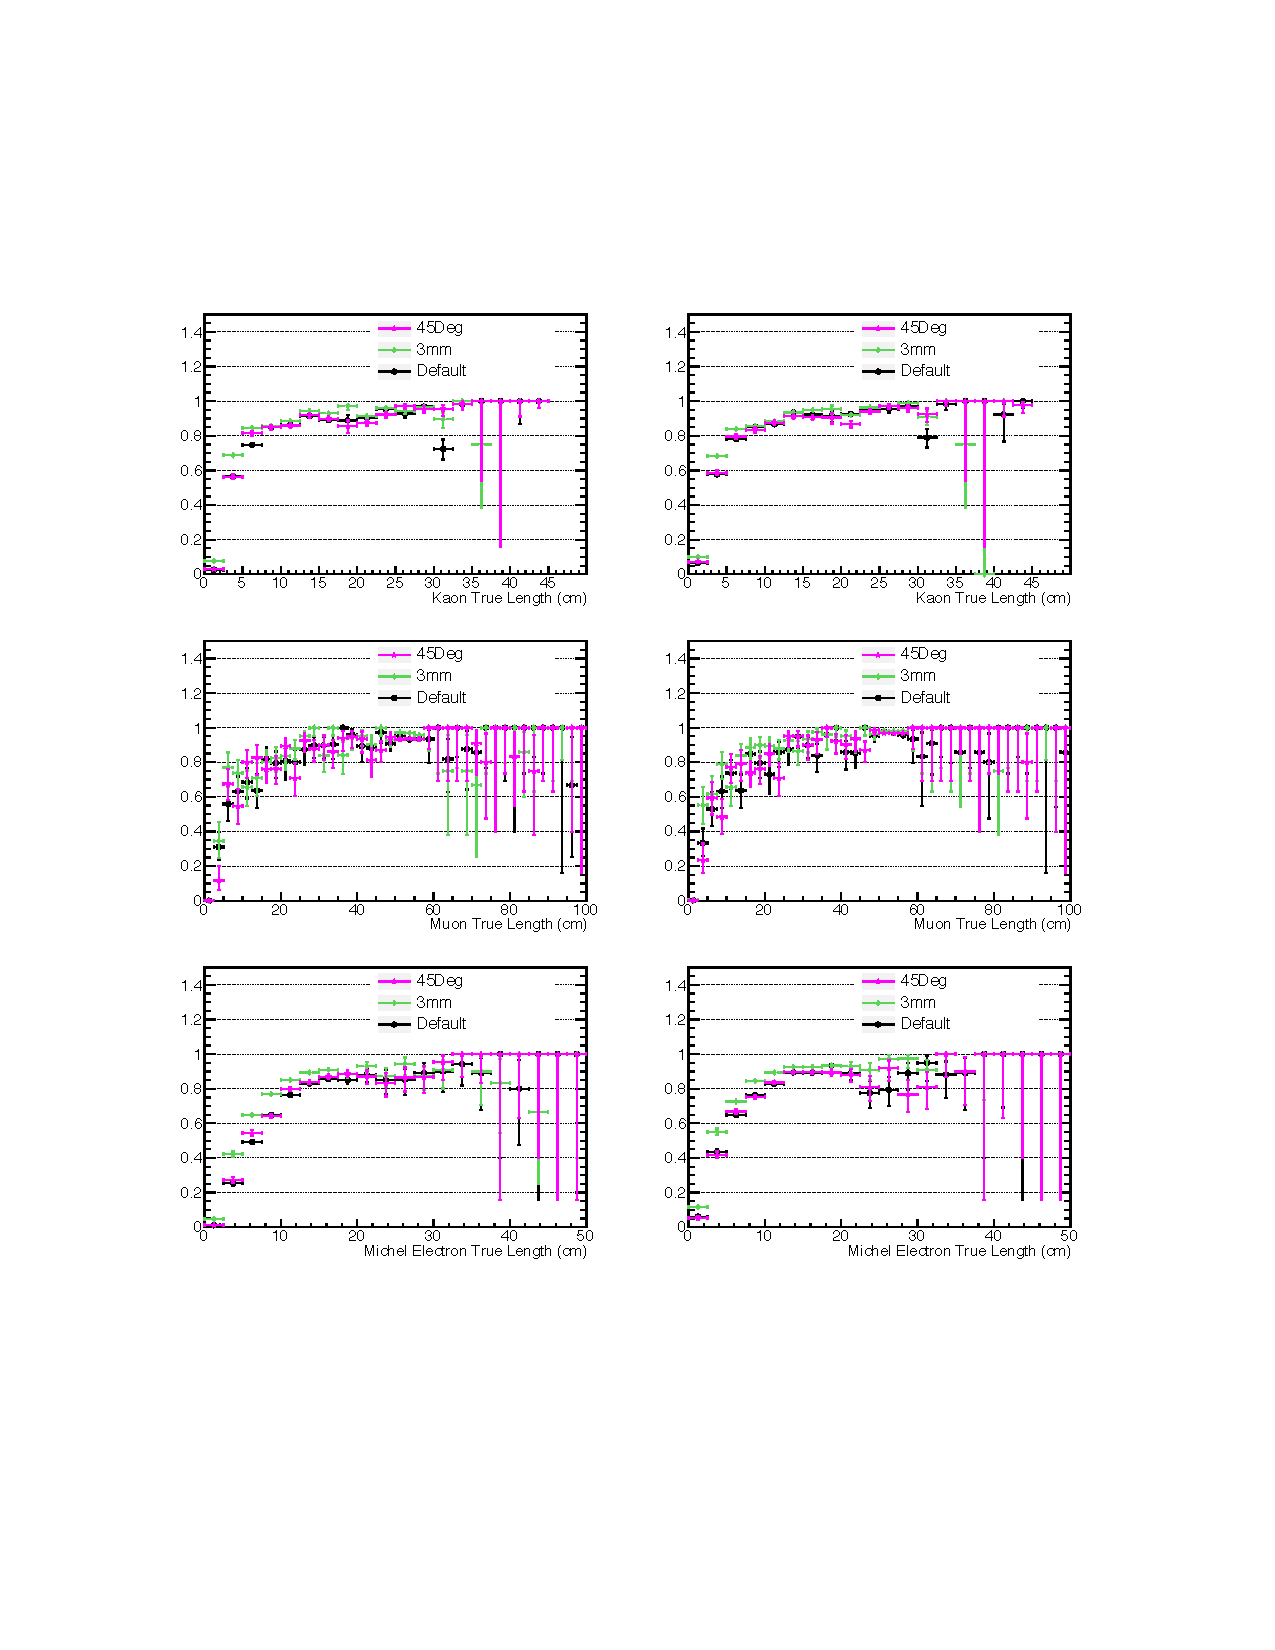
\includegraphics[width=0.85\textwidth]{TrackingEfficiency_GeometryOptimization_TwoAlgorithms.pdf}
\end{dunefigure}

\subsection{Electron and Photon Reconstruction}
\label{sec:fdsp-perform-showerreco}

\begin{dunefigure}[Impact of APA geometry on electron/photon dE/dx reconstruction]{fig:fdsp-perform_dEdx_optimization}{Average dE/dx for electrons and photons, shown for 3 arrangements of DUNE APA  geometry.}
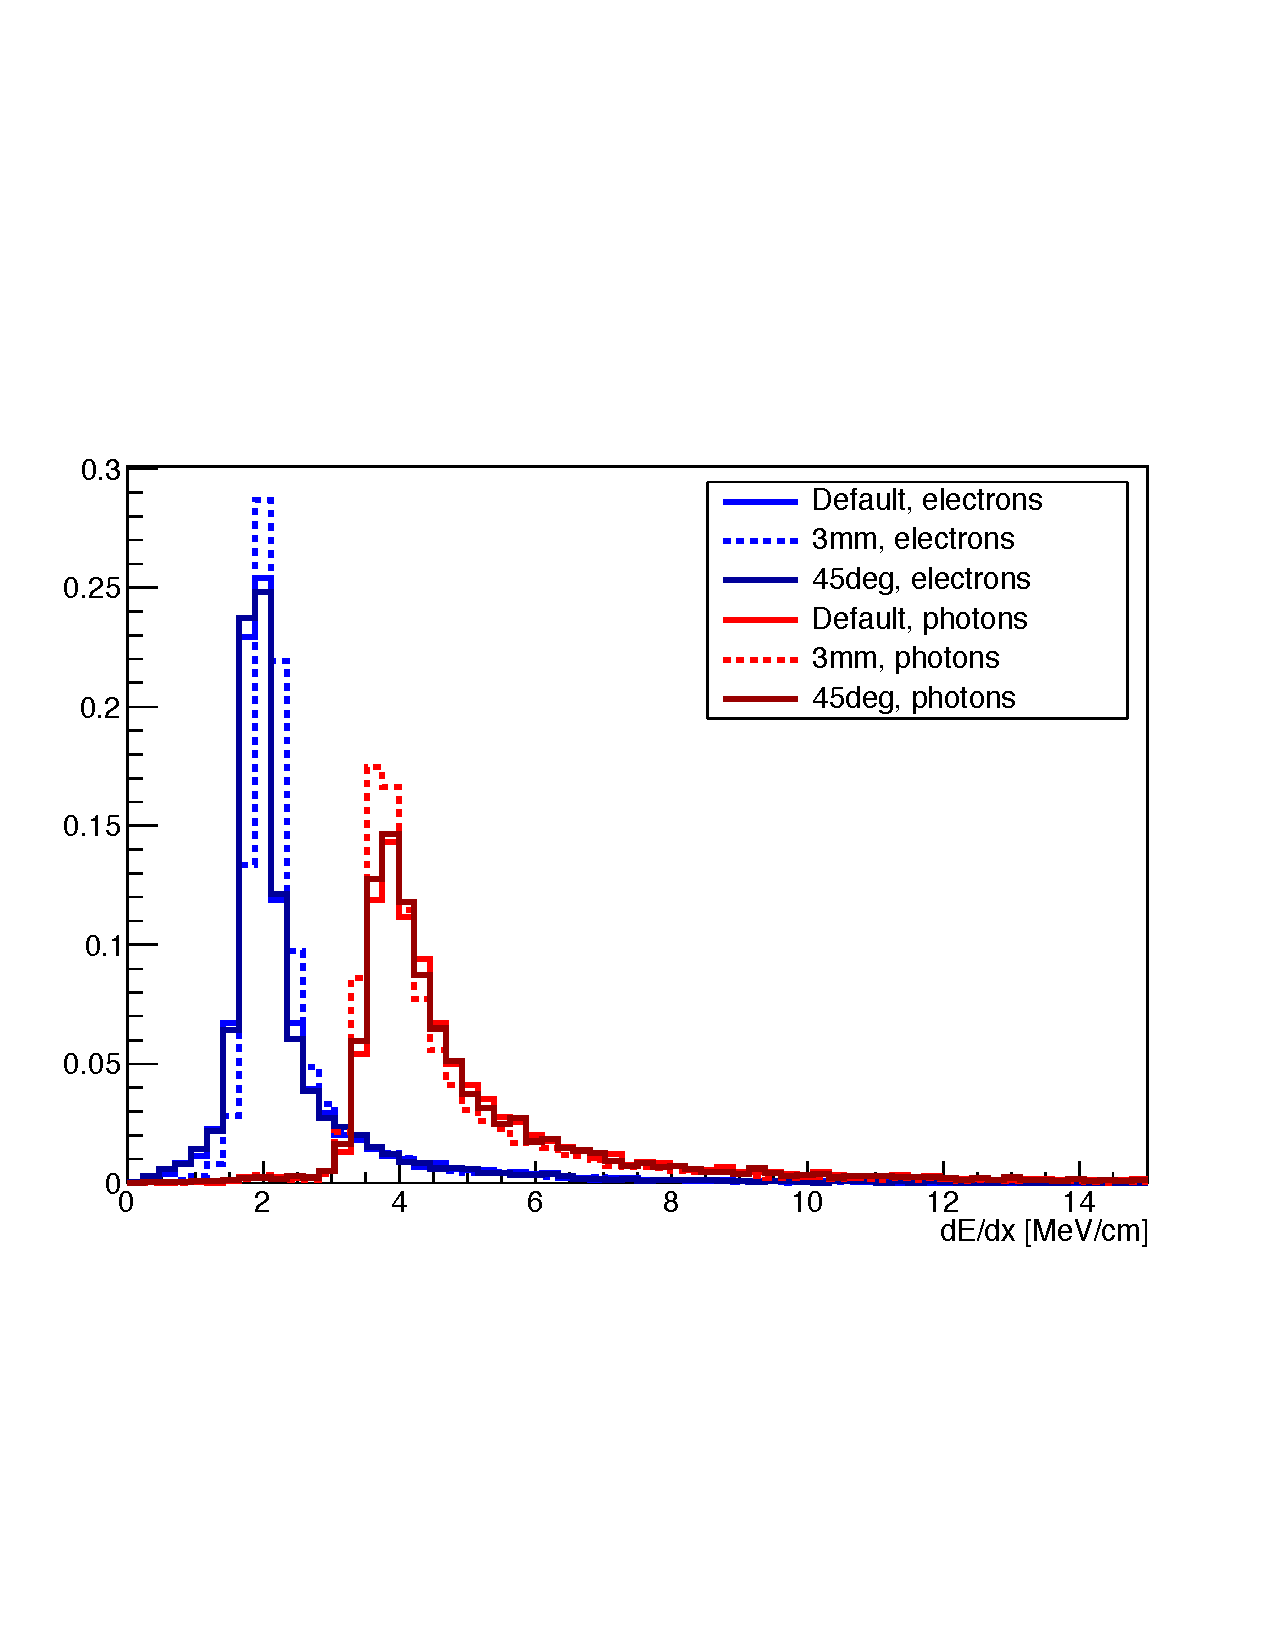
\includegraphics[width=0.6\textwidth]{dEdx.pdf}
\end{dunefigure}

\begin{dunefigure}[Impact of APA geometry on electron efficiency and photon rejection.]{fig:fdsp-perform_dEdx_optimization}{Impact of APA geometry on electron efficiency and photon rejection using a dE/dx vs. range selection approach.  Three APA configurations are shown.  The right plot is a zoomed-in view of the left plot.}
%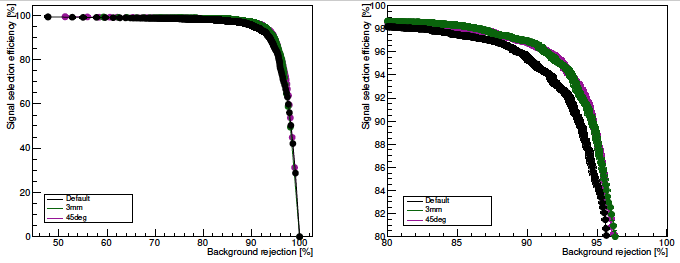
\includegraphics[width=0.85\textwidth]{egamma_signalbackground_optimization.pdf}  reduce file size on image by DeMuth
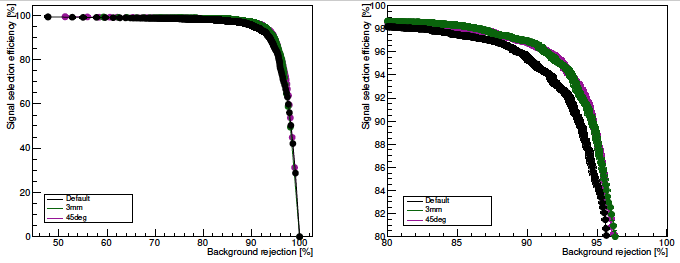
\includegraphics[width=0.85\textwidth]{egamma_signalbackground_optimization.png}
\end{dunefigure}


\section{Lessons Learned for Single-Phase LArTPCs}
\label{sec:fdsp-perform-lessons}

DUNE-SP benefits from the collective experience of several previous LArTPC detectors, and many important lessons learned from those efforts have helped shape the design of the experiment.  Among these lessons are:

\begin{itemize}
\item{Improved knowledge of achieving and maintaining high-purity LAr.}
\item{Improved understanding of the impact of LAr purity on HV system performance.}
\item{Mitigation of high-voltage discharge damage through cathode design and surge-protection elements on the field-cage.}
\item{Offline software filtering to improve electronics signal/noise levels.}
\item{Anode design to protect against broken/shorted wires.}
\end{itemize}

\subsection{Impact of Operating Drift-Field}
\label{sec:fdsp-perform-drift}

The very long drift lengths inherent in the DUNE-SP design require that the combination of drift electric field and LAr purity are sufficient to minimize charge attenuation throughout the TPC.  The nominal operating electric field in the detector if 0.5 kV/cm, which corresponds to an electron drift-velocity of 1.5 mm/$\mu$s, as shown in Figure \ref{fig:fdsp-perform_driftfield}.  An electron drifting over the full 3.6 m length of the TPC will require 2.4 ms to travel that distance under those conditions.  If the electron lifetime of the LAr in the TPC is at the 3.0 ms level, then an attenuation of approximately 50$\%$ should be anticipated for these longest drift lengths, as shown in Figure \ref{fig:fdsp-perform_attenuation}.


\begin{dunefigure}[Drift field vs. drift velocity]{fig:fdsp-perform_driftfield}{The ionization drift-velocity in LAr as a function of the electric field present in the LArTPC, for three different values of LAr temperature.  Measured data from the ICARUS experiment is overlaid.}
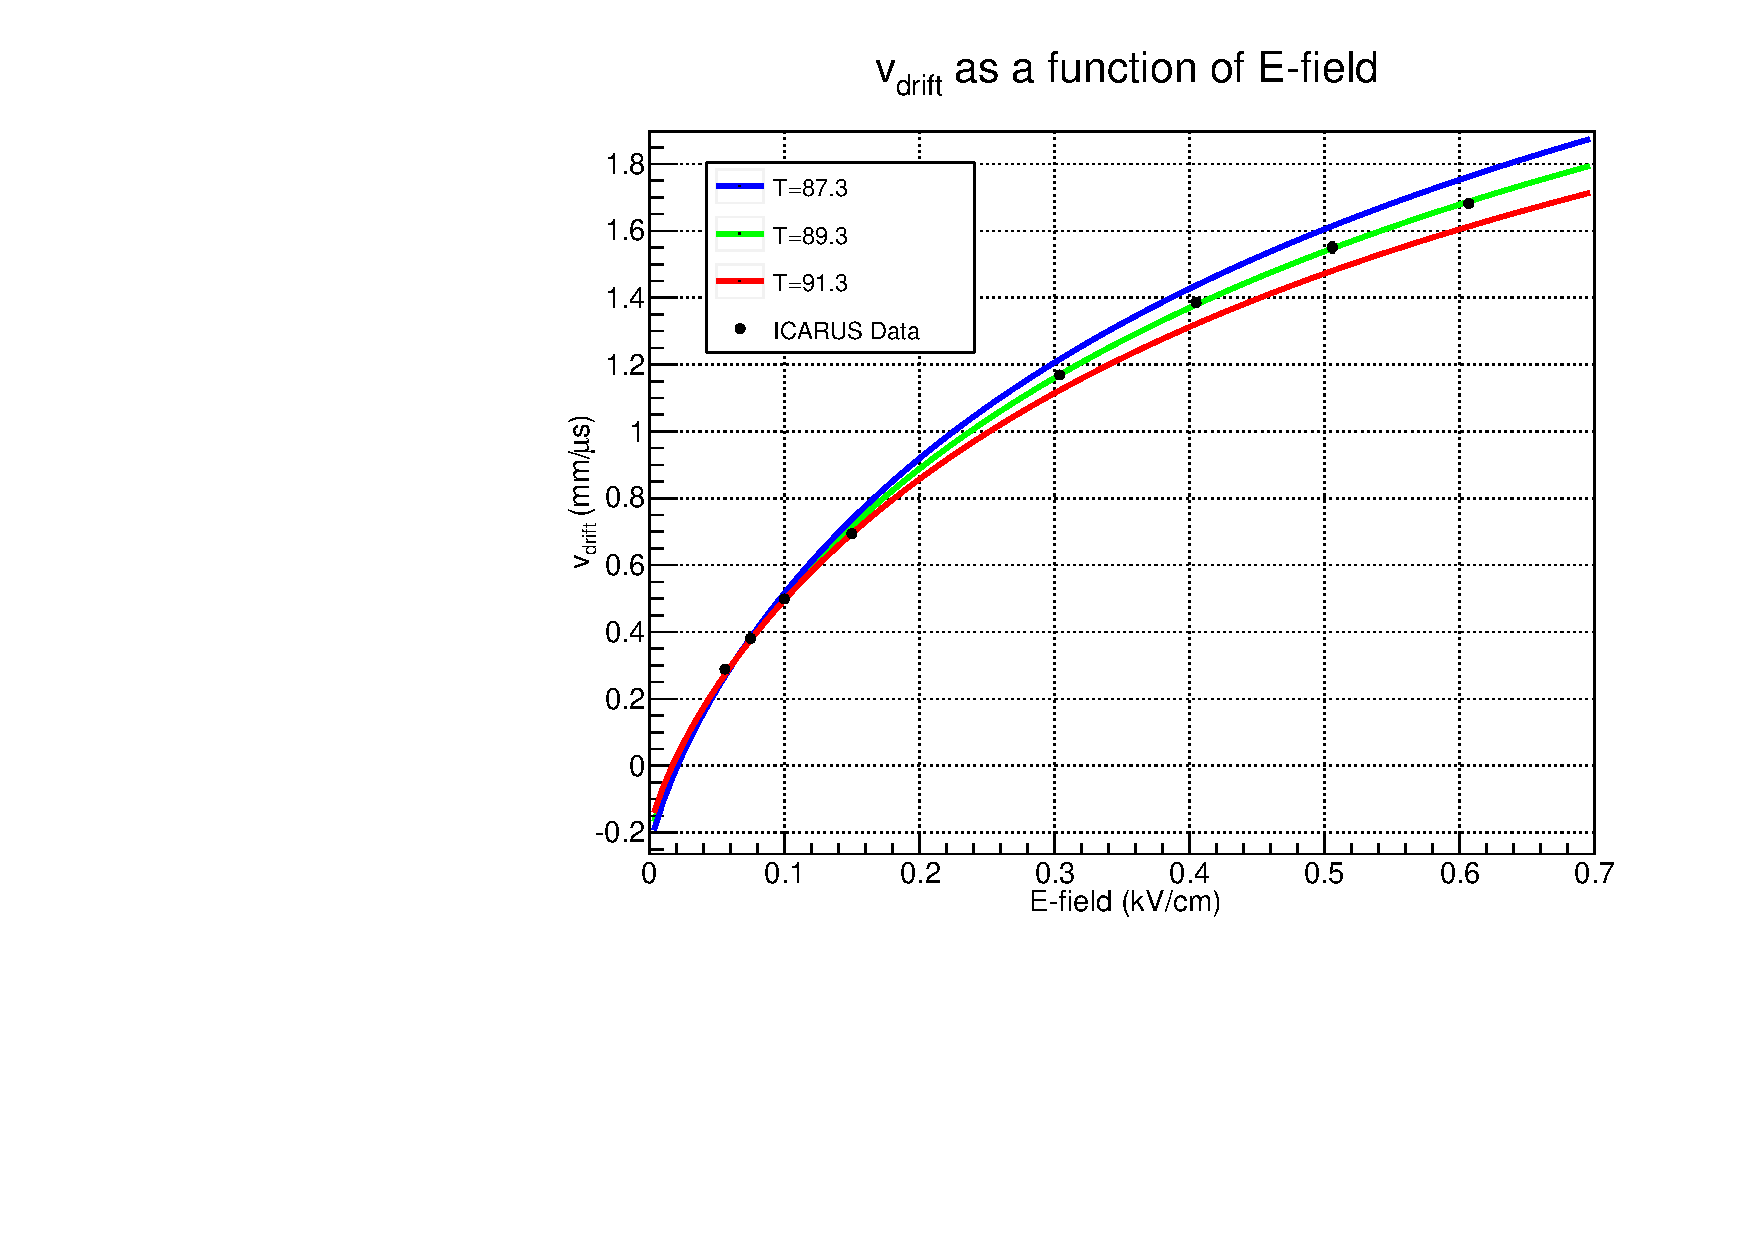
\includegraphics[width=0.6\textwidth]{DriftField_Vs_Velocity.pdf}
\end{dunefigure}

\begin{dunefigure}[Electron lifetime impact on free electron attenuation]{fig:fdsp-perform_attenuation}{The percentage of free electron attenuation as a function  of the drift length of the electron, shown for several values of electron lifetime.}
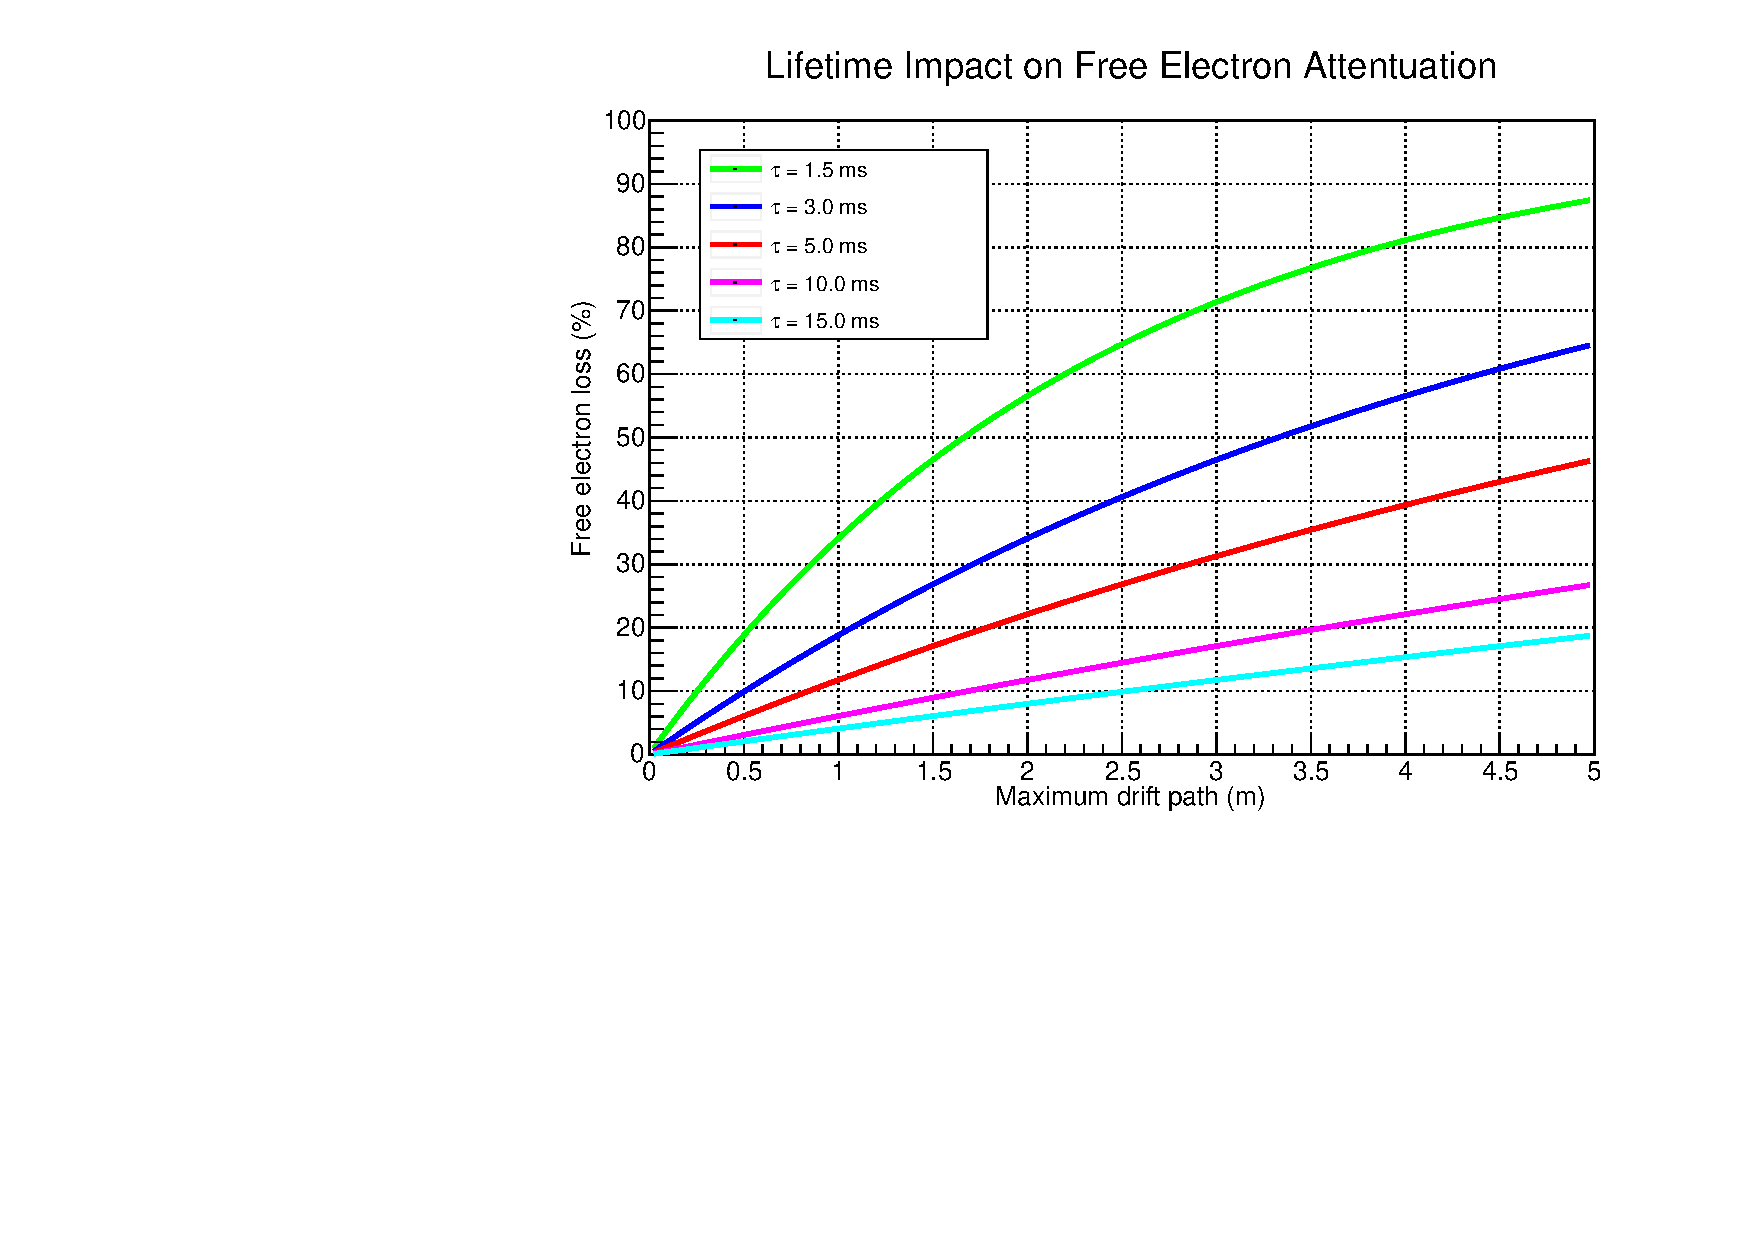
\includegraphics[width=0.6\textwidth]{Lifetime_vs_Attenuation.pdf}
\end{dunefigure}

\subsection{Impact of Electronic Noise and Missing Channels}
\label{sec:fdsp-perform-noise}

\begin{dunefigure}[Noise filtering in MicroBooNE LArTPC]{fig:fdsp-perform_noisefilter}{Reproduction of Figure 14 from \textbf{CITE MicroBooNE Noise Paper}, showing raw LArTPC signal (a) before and (b) after offline noise filtering.}
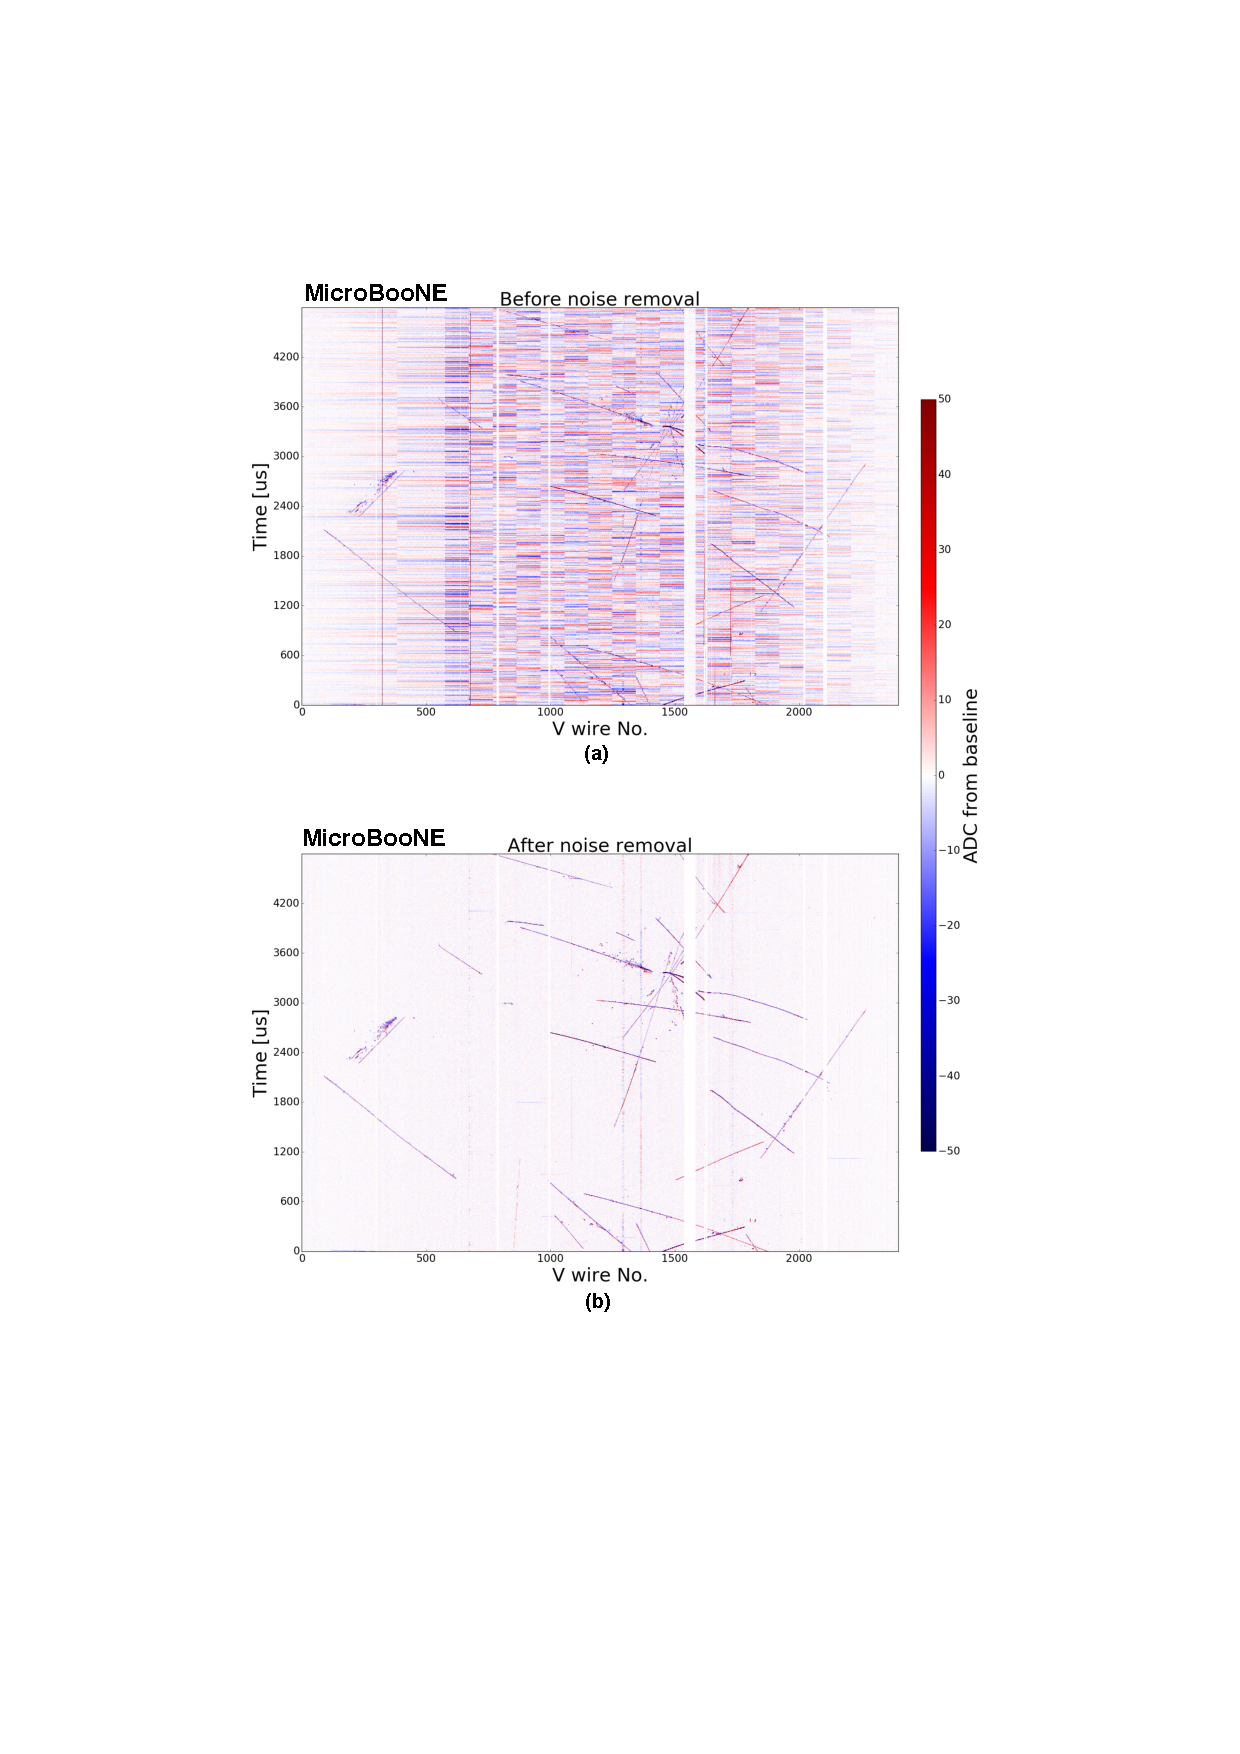
\includegraphics[width=0.85\textwidth]{NoiseFiltering_MicroBooNE.pdf}
\end{dunefigure}
